\documentclass[1p]{elsarticle_modified}
%\bibliographystyle{elsarticle-num}

%\usepackage[colorlinks]{hyperref}
%\usepackage{abbrmath_seonhwa} %\Abb, \Ascr, \Acal ,\Abf, \Afrak
\usepackage{amsfonts}
\usepackage{amssymb}
\usepackage{amsmath}
\usepackage{amsthm}
\usepackage{scalefnt}
\usepackage{amsbsy}
\usepackage{kotex}
\usepackage{caption}
\usepackage{subfig}
\usepackage{color}
\usepackage{graphicx}
\usepackage{xcolor} %% white, black, red, green, blue, cyan, magenta, yellow
\usepackage{float}
\usepackage{setspace}
\usepackage{hyperref}

\usepackage{tikz}
\usetikzlibrary{arrows}

\usepackage{multirow}
\usepackage{array} % fixed length table
\usepackage{hhline}

%%%%%%%%%%%%%%%%%%%%%
\makeatletter
\renewcommand*\env@matrix[1][\arraystretch]{%
	\edef\arraystretch{#1}%
	\hskip -\arraycolsep
	\let\@ifnextchar\new@ifnextchar
	\array{*\c@MaxMatrixCols c}}
\makeatother %https://tex.stackexchange.com/questions/14071/how-can-i-increase-the-line-spacing-in-a-matrix
%%%%%%%%%%%%%%%

\usepackage[normalem]{ulem}

\newcommand{\msout}[1]{\ifmmode\text{\sout{\ensuremath{#1}}}\else\sout{#1}\fi}
%SOURCE: \msout is \stkout macro in https://tex.stackexchange.com/questions/20609/strikeout-in-math-mode

\newcommand{\cancel}[1]{
	\ifmmode
	{\color{red}\msout{#1}}
	\else
	{\color{red}\sout{#1}}
	\fi
}

\newcommand{\add}[1]{
	{\color{blue}\uwave{#1}}
}

\newcommand{\replace}[2]{
	\ifmmode
	{\color{red}\msout{#1}}{\color{blue}\uwave{#2}}
	\else
	{\color{red}\sout{#1}}{\color{blue}\uwave{#2}}
	\fi
}

\newcommand{\Sol}{\mathcal{S}} %segment
\newcommand{\D}{D} %diagram
\newcommand{\A}{\mathcal{A}} %arc


%%%%%%%%%%%%%%%%%%%%%%%%%%%%%5 test

\def\sl{\operatorname{\textup{SL}}(2,\Cbb)}
\def\psl{\operatorname{\textup{PSL}}(2,\Cbb)}
\def\quan{\mkern 1mu \triangleright \mkern 1mu}

\theoremstyle{definition}
\newtheorem{thm}{Theorem}[section]
\newtheorem{prop}[thm]{Proposition}
\newtheorem{lem}[thm]{Lemma}
\newtheorem{ques}[thm]{Question}
\newtheorem{cor}[thm]{Corollary}
\newtheorem{defn}[thm]{Definition}
\newtheorem{exam}[thm]{Example}
\newtheorem{rmk}[thm]{Remark}
\newtheorem{alg}[thm]{Algorithm}

\newcommand{\I}{\sqrt{-1}}
\begin{document}

%\begin{frontmatter}
%
%\title{Boundary parabolic representations of knots up to 8 crossings}
%
%%% Group authors per affiliation:
%\author{Yunhi Cho} 
%\address{Department of Mathematics, University of Seoul, Seoul, Korea}
%\ead{yhcho@uos.ac.kr}
%
%
%\author{Seonhwa Kim} %\fnref{s_kim}}
%\address{Center for Geometry and Physics, Institute for Basic Science, Pohang, 37673, Korea}
%\ead{ryeona17@ibs.re.kr}
%
%\author{Hyuk Kim}
%\address{Department of Mathematical Sciences, Seoul National University, Seoul 08826, Korea}
%\ead{hyukkim@snu.ac.kr}
%
%\author{Seokbeom Yoon}
%\address{Department of Mathematical Sciences, Seoul National University, Seoul, 08826,  Korea}
%\ead{sbyoon15@snu.ac.kr}
%
%\begin{abstract}
%We find all boundary parabolic representation of knots up to 8 crossings.
%
%\end{abstract}
%\begin{keyword}
%    \MSC[2010] 57M25 
%\end{keyword}
%
%\end{frontmatter}

%\linenumbers
%\tableofcontents
%
\newcommand\colored[1]{\textcolor{white}{\rule[-0.35ex]{0.8em}{1.4ex}}\kern-0.8em\color{red} #1}%
%\newcommand\colored[1]{\textcolor{white}{ #1}\kern-2.17ex	\textcolor{white}{ #1}\kern-1.81ex	\textcolor{white}{ #1}\kern-2.15ex\color{red}#1	}

{\Large $\underline{12n_{0773}~(K12n_{0773})}$}

\setlength{\tabcolsep}{10pt}
\renewcommand{\arraystretch}{1.6}
\vspace{1cm}\begin{tabular}{m{100pt}>{\centering\arraybackslash}m{274pt}}
\multirow{5}{120pt}{
	\centering
	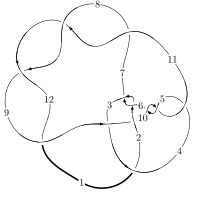
\includegraphics[width=112pt]{../../../GIT/diagram.site/Diagrams/png/2862_12n_0773.png}\\
\ \ \ A knot diagram\footnotemark}&
\allowdisplaybreaks
\textbf{Linearized knot diagam} \\
\cline{2-2}
 &
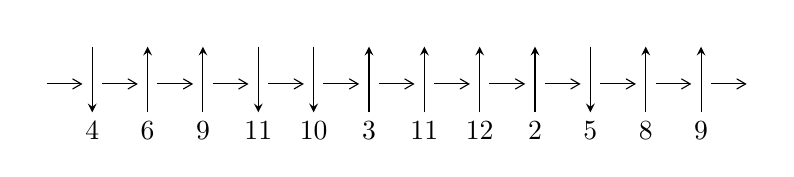
\begin{tikzpicture}[x=20pt, y=17pt]
	% nodes
	\node (C0) at (0, 0) {};
	\node (C1) at (1, 0) {};
	\node (C1U) at (1, +1) {};
	\node (C1D) at (1, -1) {4};

	\node (C2) at (2, 0) {};
	\node (C2U) at (2, +1) {};
	\node (C2D) at (2, -1) {6};

	\node (C3) at (3, 0) {};
	\node (C3U) at (3, +1) {};
	\node (C3D) at (3, -1) {9};

	\node (C4) at (4, 0) {};
	\node (C4U) at (4, +1) {};
	\node (C4D) at (4, -1) {11};

	\node (C5) at (5, 0) {};
	\node (C5U) at (5, +1) {};
	\node (C5D) at (5, -1) {10};

	\node (C6) at (6, 0) {};
	\node (C6U) at (6, +1) {};
	\node (C6D) at (6, -1) {3};

	\node (C7) at (7, 0) {};
	\node (C7U) at (7, +1) {};
	\node (C7D) at (7, -1) {11};

	\node (C8) at (8, 0) {};
	\node (C8U) at (8, +1) {};
	\node (C8D) at (8, -1) {12};

	\node (C9) at (9, 0) {};
	\node (C9U) at (9, +1) {};
	\node (C9D) at (9, -1) {2};

	\node (C10) at (10, 0) {};
	\node (C10U) at (10, +1) {};
	\node (C10D) at (10, -1) {5};

	\node (C11) at (11, 0) {};
	\node (C11U) at (11, +1) {};
	\node (C11D) at (11, -1) {8};

	\node (C12) at (12, 0) {};
	\node (C12U) at (12, +1) {};
	\node (C12D) at (12, -1) {9};
	\node (C13) at (13, 0) {};

	% arrows
	\draw[->,>={angle 60}]
	(C0) edge (C1) (C1) edge (C2) (C2) edge (C3) (C3) edge (C4) (C4) edge (C5) (C5) edge (C6) (C6) edge (C7) (C7) edge (C8) (C8) edge (C9) (C9) edge (C10) (C10) edge (C11) (C11) edge (C12) (C12) edge (C13) ;	\draw[->,>=stealth]
	(C1U) edge (C1D) (C2D) edge (C2U) (C3D) edge (C3U) (C4U) edge (C4D) (C5U) edge (C5D) (C6D) edge (C6U) (C7D) edge (C7U) (C8D) edge (C8U) (C9D) edge (C9U) (C10U) edge (C10D) (C11D) edge (C11U) (C12D) edge (C12U) ;
	\end{tikzpicture} \\
\hhline{~~} \\& 
\textbf{Solving Sequence} \\ \cline{2-2} 
 &
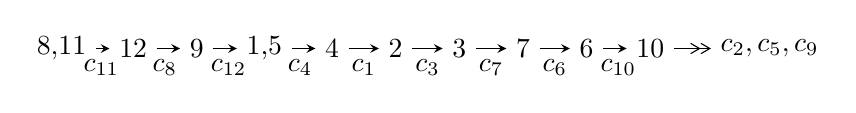
\begin{tikzpicture}[x=23pt, y=7pt]
	% node
	\node (A0) at (-1/8, 0) {8,11};
	\node (A1) at (1, 0) {12};
	\node (A2) at (2, 0) {9};
	\node (A3) at (49/16, 0) {1,5};
	\node (A4) at (33/8, 0) {4};
	\node (A5) at (41/8, 0) {2};
	\node (A6) at (49/8, 0) {3};
	\node (A7) at (57/8, 0) {7};
	\node (A8) at (65/8, 0) {6};
	\node (A9) at (73/8, 0) {10};
	\node (C1) at (1/2, -1) {$c_{11}$};
	\node (C2) at (3/2, -1) {$c_{8}$};
	\node (C3) at (5/2, -1) {$c_{12}$};
	\node (C4) at (29/8, -1) {$c_{4}$};
	\node (C5) at (37/8, -1) {$c_{1}$};
	\node (C6) at (45/8, -1) {$c_{3}$};
	\node (C7) at (53/8, -1) {$c_{7}$};
	\node (C8) at (61/8, -1) {$c_{6}$};
	\node (C9) at (69/8, -1) {$c_{10}$};
	\node (A10) at (11, 0) {$c_{2},c_{5},c_{9}$};

	% edge
	\draw[->,>=stealth]	
	(A0) edge (A1) (A1) edge (A2) (A2) edge (A3) (A3) edge (A4) (A4) edge (A5) (A5) edge (A6) (A6) edge (A7) (A7) edge (A8) (A8) edge (A9) ;
	\draw[->>,>={angle 60}]	
	(A9) edge (A10);
\end{tikzpicture} \\ 

\end{tabular} \\

\footnotetext{
The image of knot diagram is generated by the software ``\textbf{Draw programme}" developed by Andrew Bartholomew(\url{http://www.layer8.co.uk/maths/draw/index.htm\#Running-draw}), where we modified some parts for our purpose(\url{https://github.com/CATsTAILs/LinksPainter}).
}\phantom \\ \newline 
\centering \textbf{Ideals for irreducible components\footnotemark of $X_{\text{par}}$} 
 
\begin{align*}
I^u_{1}&=\langle 
-2.99252\times10^{54} u^{58}-4.27398\times10^{53} u^{57}+\cdots+1.08123\times10^{55} b-5.85001\times10^{54},\\
\phantom{I^u_{1}}&\phantom{= \langle  }-8.90269\times10^{54} u^{58}+1.21104\times10^{55} u^{57}+\cdots+1.08123\times10^{55} a-4.30153\times10^{56},\;u^{59}- u^{58}+\cdots+32 u+1\rangle \\
I^u_{2}&=\langle 
2 u^{14}- u^{13}-16 u^{12}+8 u^{11}+49 u^{10}-26 u^9-67 u^8+42 u^7+27 u^6-31 u^5+22 u^4+7 u^3-18 u^2+b+2,\\
\phantom{I^u_{2}}&\phantom{= \langle  }-2 u^{14}+2 u^{13}+\cdots+a+1,\\
\phantom{I^u_{2}}&\phantom{= \langle  }u^{15}-9 u^{13}+32 u^{11}- u^{10}-55 u^9+6 u^8+41 u^7-13 u^6+13 u^4-13 u^3-6 u^2+2 u+1\rangle \\
\\
\end{align*}
\raggedright * 2 irreducible components of $\dim_{\mathbb{C}}=0$, with total 74 representations.\\
\footnotetext{All coefficients of polynomials are rational numbers. But the coefficients are sometimes approximated in decimal forms when there is not enough margin.}
\newpage
\renewcommand{\arraystretch}{1}
\centering \section*{I. $I^u_{1}= \langle -2.99\times10^{54} u^{58}-4.27\times10^{53} u^{57}+\cdots+1.08\times10^{55} b-5.85\times10^{54},\;-8.90\times10^{54} u^{58}+1.21\times10^{55} u^{57}+\cdots+1.08\times10^{55} a-4.30\times10^{56},\;u^{59}- u^{58}+\cdots+32 u+1 \rangle$}
\flushleft \textbf{(i) Arc colorings}\\
\begin{tabular}{m{7pt} m{180pt} m{7pt} m{180pt} }
\flushright $a_{8}=$&$\begin{pmatrix}0\\u\end{pmatrix}$ \\
\flushright $a_{11}=$&$\begin{pmatrix}1\\0\end{pmatrix}$ \\
\flushright $a_{12}=$&$\begin{pmatrix}1\\- u^2\end{pmatrix}$ \\
\flushright $a_{9}=$&$\begin{pmatrix}u\\- u^3+u\end{pmatrix}$ \\
\flushright $a_{1}=$&$\begin{pmatrix}- u^2+1\\u^4-2 u^2\end{pmatrix}$ \\
\flushright $a_{5}=$&$\begin{pmatrix}0.823385 u^{58}-1.12006 u^{57}+\cdots-182.375 u+39.7837\\0.276770 u^{58}+0.0395289 u^{57}+\cdots-0.767568 u+0.541051\end{pmatrix}$ \\
\flushright $a_{4}=$&$\begin{pmatrix}1.10016 u^{58}-1.08053 u^{57}+\cdots-183.142 u+40.3248\\0.276770 u^{58}+0.0395289 u^{57}+\cdots-0.767568 u+0.541051\end{pmatrix}$ \\
\flushright $a_{2}=$&$\begin{pmatrix}-0.483130 u^{58}-1.09918 u^{57}+\cdots-102.939 u+26.7972\\0.581937 u^{58}+0.395648 u^{57}+\cdots-24.3369 u-0.367973\end{pmatrix}$ \\
\flushright $a_{3}=$&$\begin{pmatrix}1.22082 u^{58}-0.989380 u^{57}+\cdots-182.255 u+40.3858\\-0.00126625 u^{58}-0.0204342 u^{57}+\cdots+7.01822 u+0.813889\end{pmatrix}$ \\
\flushright $a_{7}=$&$\begin{pmatrix}- u\\u\end{pmatrix}$ \\
\flushright $a_{6}=$&$\begin{pmatrix}1.84485 u^{58}-1.31590 u^{57}+\cdots-229.979 u+52.0102\\-0.472356 u^{58}-0.328224 u^{57}+\cdots+6.26065 u+0.900727\end{pmatrix}$ \\
\flushright $a_{10}=$&$\begin{pmatrix}-1.94402 u^{58}+0.476904 u^{57}+\cdots+139.733 u-20.1503\\0.316358 u^{58}-0.0242382 u^{57}+\cdots+0.806174 u-0.303933\end{pmatrix}$\\&\end{tabular}
\flushleft \textbf{(ii) Obstruction class $= -1$}\\~\\
\flushleft \textbf{(iii) Cusp Shapes $= 1.27874 u^{58}+0.721176 u^{57}+\cdots-64.5120 u-5.58630$}\\~\\
\newpage\renewcommand{\arraystretch}{1}
\flushleft \textbf{(iv) u-Polynomials at the component}\newline \\
\begin{tabular}{m{50pt}|m{274pt}}
Crossings & \hspace{64pt}u-Polynomials at each crossing \\
\hline $$\begin{aligned}c_{1}\end{aligned}$$&$\begin{aligned}
&u^{59}-9 u^{58}+\cdots-108 u+61
\end{aligned}$\\
\hline $$\begin{aligned}c_{2},c_{6}\end{aligned}$$&$\begin{aligned}
&u^{59}-2 u^{58}+\cdots+5154 u-773
\end{aligned}$\\
\hline $$\begin{aligned}c_{3}\end{aligned}$$&$\begin{aligned}
&u^{59}- u^{58}+\cdots+23 u-43
\end{aligned}$\\
\hline $$\begin{aligned}c_{4},c_{5},c_{10}\end{aligned}$$&$\begin{aligned}
&u^{59}- u^{58}+\cdots+102 u+1
\end{aligned}$\\
\hline $$\begin{aligned}c_{7},c_{8},c_{11}\\c_{12}\end{aligned}$$&$\begin{aligned}
&u^{59}- u^{58}+\cdots+32 u+1
\end{aligned}$\\
\hline $$\begin{aligned}c_{9}\end{aligned}$$&$\begin{aligned}
&u^{59}+2 u^{58}+\cdots+1624 u-1291
\end{aligned}$\\
\hline
\end{tabular}\\~\\
\newpage\renewcommand{\arraystretch}{1}
\flushleft \textbf{(v) Riley Polynomials at the component}\newline \\
\begin{tabular}{m{50pt}|m{274pt}}
Crossings & \hspace{64pt}Riley Polynomials at each crossing \\
\hline $$\begin{aligned}c_{1}\end{aligned}$$&$\begin{aligned}
&y^{59}-33 y^{58}+\cdots+229434 y-3721
\end{aligned}$\\
\hline $$\begin{aligned}c_{2},c_{6}\end{aligned}$$&$\begin{aligned}
&y^{59}-40 y^{58}+\cdots+18677570 y-597529
\end{aligned}$\\
\hline $$\begin{aligned}c_{3}\end{aligned}$$&$\begin{aligned}
&y^{59}+31 y^{58}+\cdots-87965 y-1849
\end{aligned}$\\
\hline $$\begin{aligned}c_{4},c_{5},c_{10}\end{aligned}$$&$\begin{aligned}
&y^{59}+59 y^{58}+\cdots+10138 y-1
\end{aligned}$\\
\hline $$\begin{aligned}c_{7},c_{8},c_{11}\\c_{12}\end{aligned}$$&$\begin{aligned}
&y^{59}-53 y^{58}+\cdots+1298 y-1
\end{aligned}$\\
\hline $$\begin{aligned}c_{9}\end{aligned}$$&$\begin{aligned}
&y^{59}-32 y^{58}+\cdots+37592492 y-1666681
\end{aligned}$\\
\hline
\end{tabular}\\~\\
\newpage\flushleft \textbf{(vi) Complex Volumes and Cusp Shapes}
$$\begin{array}{c|c|c}  
\text{Solutions to }I^u_{1}& \I (\text{vol} + \sqrt{-1}CS) & \text{Cusp shape}\\
 \hline 
\begin{aligned}
u &= -0.264830 + 0.931382 I \\
a &= -0.880909 + 0.866071 I \\
b &= -0.36110 - 1.47905 I\end{aligned}
 & \phantom{-}3.66563 - 9.89323 I & \phantom{-}7.43337 + 6.27116 I \\ \hline\begin{aligned}
u &= -0.264830 - 0.931382 I \\
a &= -0.880909 - 0.866071 I \\
b &= -0.36110 + 1.47905 I\end{aligned}
 & \phantom{-}3.66563 + 9.89323 I & \phantom{-}7.43337 - 6.27116 I \\ \hline\begin{aligned}
u &= \phantom{-}0.119168 + 0.889846 I \\
a &= -0.474592 - 0.195483 I \\
b &= -0.924980 + 0.347695 I\end{aligned}
 & -2.19237 + 5.25619 I & \phantom{-}4.23819 - 5.61197 I \\ \hline\begin{aligned}
u &= \phantom{-}0.119168 - 0.889846 I \\
a &= -0.474592 + 0.195483 I \\
b &= -0.924980 - 0.347695 I\end{aligned}
 & -2.19237 - 5.25619 I & \phantom{-}4.23819 + 5.61197 I \\ \hline\begin{aligned}
u &= -0.056257 + 0.894737 I \\
a &= \phantom{-}0.654957 - 0.276427 I \\
b &= \phantom{-}0.165353 + 1.327120 I\end{aligned}
 & \phantom{-}0.33927 - 2.65716 I & \phantom{-}7.07647 + 3.01945 I \\ \hline\begin{aligned}
u &= -0.056257 - 0.894737 I \\
a &= \phantom{-}0.654957 + 0.276427 I \\
b &= \phantom{-}0.165353 - 1.327120 I\end{aligned}
 & \phantom{-}0.33927 + 2.65716 I & \phantom{-}7.07647 - 3.01945 I \\ \hline\begin{aligned}
u &= \phantom{-}1.110480 + 0.149176 I \\
a &= -0.444606 + 1.134310 I \\
b &= -0.394307 - 0.923884 I\end{aligned}
 & \phantom{-}1.42201 + 0.91602 I & \phantom{-0.000000 } 0 \\ \hline\begin{aligned}
u &= \phantom{-}1.110480 - 0.149176 I \\
a &= -0.444606 - 1.134310 I \\
b &= -0.394307 + 0.923884 I\end{aligned}
 & \phantom{-}1.42201 - 0.91602 I & \phantom{-0.000000 } 0 \\ \hline\begin{aligned}
u &= \phantom{-}0.876618\phantom{ +0.000000I} \\
a &= -0.237869\phantom{ +0.000000I} \\
b &= \phantom{-}0.547477\phantom{ +0.000000I}\end{aligned}
 & \phantom{-}1.47441\phantom{ +0.000000I} & \phantom{-}6.10400\phantom{ +0.000000I} \\ \hline\begin{aligned}
u &= -0.946025 + 0.638857 I \\
a &= -0.59515 + 1.28359 I \\
b &= \phantom{-}0.31286 - 1.38423 I\end{aligned}
 & \phantom{-}5.77333 + 4.51012 I & \phantom{-0.000000 } 0\\
 \hline 
 \end{array}$$\newpage$$\begin{array}{c|c|c}  
\text{Solutions to }I^u_{1}& \I (\text{vol} + \sqrt{-1}CS) & \text{Cusp shape}\\
 \hline 
\begin{aligned}
u &= -0.946025 - 0.638857 I \\
a &= -0.59515 - 1.28359 I \\
b &= \phantom{-}0.31286 + 1.38423 I\end{aligned}
 & \phantom{-}5.77333 - 4.51012 I & \phantom{-0.000000 } 0 \\ \hline\begin{aligned}
u &= -1.140520 + 0.188136 I \\
a &= \phantom{-}0.22857 - 1.65457 I \\
b &= \phantom{-}0.284860 + 0.755221 I\end{aligned}
 & \phantom{-}3.89321 - 2.91811 I & \phantom{-0.000000 } 0 \\ \hline\begin{aligned}
u &= -1.140520 - 0.188136 I \\
a &= \phantom{-}0.22857 + 1.65457 I \\
b &= \phantom{-}0.284860 - 0.755221 I\end{aligned}
 & \phantom{-}3.89321 + 2.91811 I & \phantom{-0.000000 } 0 \\ \hline\begin{aligned}
u &= -0.102126 + 0.801805 I \\
a &= \phantom{-}0.688121 - 0.400215 I \\
b &= \phantom{-}0.498536 - 0.055398 I\end{aligned}
 & -4.03916 + 0.26803 I & -0.184983 + 0.165110 I \\ \hline\begin{aligned}
u &= -0.102126 - 0.801805 I \\
a &= \phantom{-}0.688121 + 0.400215 I \\
b &= \phantom{-}0.498536 + 0.055398 I\end{aligned}
 & -4.03916 - 0.26803 I & -0.184983 - 0.165110 I \\ \hline\begin{aligned}
u &= \phantom{-}0.373831 + 0.712271 I \\
a &= \phantom{-}1.14505 + 1.41925 I \\
b &= \phantom{-}0.142122 - 1.261840 I\end{aligned}
 & -0.31798 + 2.01882 I & \phantom{-}8.09002 - 3.66839 I \\ \hline\begin{aligned}
u &= \phantom{-}0.373831 - 0.712271 I \\
a &= \phantom{-}1.14505 - 1.41925 I \\
b &= \phantom{-}0.142122 + 1.261840 I\end{aligned}
 & -0.31798 - 2.01882 I & \phantom{-}8.09002 + 3.66839 I \\ \hline\begin{aligned}
u &= \phantom{-}1.115350 + 0.452791 I \\
a &= -0.361726 + 0.339593 I \\
b &= \phantom{-}0.824800 + 0.143591 I\end{aligned}
 & \phantom{-}0.891108 - 0.463329 I & \phantom{-0.000000 } 0 \\ \hline\begin{aligned}
u &= \phantom{-}1.115350 - 0.452791 I \\
a &= -0.361726 - 0.339593 I \\
b &= \phantom{-}0.824800 - 0.143591 I\end{aligned}
 & \phantom{-}0.891108 + 0.463329 I & \phantom{-0.000000 } 0 \\ \hline\begin{aligned}
u &= -1.22285\phantom{ +0.000000I} \\
a &= \phantom{-}2.11329\phantom{ +0.000000I} \\
b &= -0.00993937\phantom{ +0.000000I}\end{aligned}
 & \phantom{-}6.34821\phantom{ +0.000000I} & \phantom{-0.000000 } 0\\
 \hline 
 \end{array}$$\newpage$$\begin{array}{c|c|c}  
\text{Solutions to }I^u_{1}& \I (\text{vol} + \sqrt{-1}CS) & \text{Cusp shape}\\
 \hline 
\begin{aligned}
u &= \phantom{-}0.069536 + 0.754894 I \\
a &= -0.723962 - 0.583814 I \\
b &= -0.659233 + 0.942112 I\end{aligned}
 & -0.414783 + 0.267178 I & \phantom{-}7.48415 + 0.42381 I \\ \hline\begin{aligned}
u &= \phantom{-}0.069536 - 0.754894 I \\
a &= -0.723962 + 0.583814 I \\
b &= -0.659233 - 0.942112 I\end{aligned}
 & -0.414783 - 0.267178 I & \phantom{-}7.48415 - 0.42381 I \\ \hline\begin{aligned}
u &= \phantom{-}1.246900 + 0.128101 I \\
a &= \phantom{-}0.84306 + 3.72917 I \\
b &= \phantom{-}0.08010 - 1.59038 I\end{aligned}
 & \phantom{-}11.78010 + 4.24713 I & \phantom{-0.000000 } 0 \\ \hline\begin{aligned}
u &= \phantom{-}1.246900 - 0.128101 I \\
a &= \phantom{-}0.84306 - 3.72917 I \\
b &= \phantom{-}0.08010 + 1.59038 I\end{aligned}
 & \phantom{-}11.78010 - 4.24713 I & \phantom{-0.000000 } 0 \\ \hline\begin{aligned}
u &= -1.201700 + 0.358369 I \\
a &= -0.431364 + 0.406062 I \\
b &= -0.609338 - 0.225740 I\end{aligned}
 & -0.66555 - 4.45229 I & \phantom{-0.000000 } 0 \\ \hline\begin{aligned}
u &= -1.201700 - 0.358369 I \\
a &= -0.431364 - 0.406062 I \\
b &= -0.609338 + 0.225740 I\end{aligned}
 & -0.66555 + 4.45229 I & \phantom{-0.000000 } 0 \\ \hline\begin{aligned}
u &= \phantom{-}1.25489\phantom{ +0.000000I} \\
a &= -0.0869145\phantom{ +0.000000I} \\
b &= -1.08085\phantom{ +0.000000I}\end{aligned}
 & \phantom{-}6.69122\phantom{ +0.000000I} & \phantom{-0.000000 } 0 \\ \hline\begin{aligned}
u &= \phantom{-}1.244200 + 0.194794 I \\
a &= \phantom{-}2.26800 + 1.51808 I \\
b &= -0.014499 - 1.386050 I\end{aligned}
 & \phantom{-}11.09980 - 0.10055 I & \phantom{-0.000000 } 0 \\ \hline\begin{aligned}
u &= \phantom{-}1.244200 - 0.194794 I \\
a &= \phantom{-}2.26800 - 1.51808 I \\
b &= -0.014499 + 1.386050 I\end{aligned}
 & \phantom{-}11.09980 + 0.10055 I & \phantom{-0.000000 } 0 \\ \hline\begin{aligned}
u &= \phantom{-}1.238570 + 0.325666 I \\
a &= -0.680385 - 0.614714 I \\
b &= \phantom{-}0.919436 + 0.808126 I\end{aligned}
 & \phantom{-}3.20240 + 3.63807 I & \phantom{-0.000000 } 0\\
 \hline 
 \end{array}$$\newpage$$\begin{array}{c|c|c}  
\text{Solutions to }I^u_{1}& \I (\text{vol} + \sqrt{-1}CS) & \text{Cusp shape}\\
 \hline 
\begin{aligned}
u &= \phantom{-}1.238570 - 0.325666 I \\
a &= -0.680385 + 0.614714 I \\
b &= \phantom{-}0.919436 - 0.808126 I\end{aligned}
 & \phantom{-}3.20240 - 3.63807 I & \phantom{-0.000000 } 0 \\ \hline\begin{aligned}
u &= -1.197820 + 0.461395 I \\
a &= \phantom{-}0.413885 - 1.277320 I \\
b &= -0.062854 + 1.223650 I\end{aligned}
 & \phantom{-}3.87163 - 2.16113 I & \phantom{-0.000000 } 0 \\ \hline\begin{aligned}
u &= -1.197820 - 0.461395 I \\
a &= \phantom{-}0.413885 + 1.277320 I \\
b &= -0.062854 - 1.223650 I\end{aligned}
 & \phantom{-}3.87163 + 2.16113 I & \phantom{-0.000000 } 0 \\ \hline\begin{aligned}
u &= -1.278360 + 0.133753 I \\
a &= -0.40499 + 2.53862 I \\
b &= \phantom{-}0.15595 - 1.70029 I\end{aligned}
 & \phantom{-}12.17270 + 0.50014 I & \phantom{-0.000000 } 0 \\ \hline\begin{aligned}
u &= -1.278360 - 0.133753 I \\
a &= -0.40499 - 2.53862 I \\
b &= \phantom{-}0.15595 + 1.70029 I\end{aligned}
 & \phantom{-}12.17270 - 0.50014 I & \phantom{-0.000000 } 0 \\ \hline\begin{aligned}
u &= -1.280870 + 0.190846 I \\
a &= -0.94846 + 1.39858 I \\
b &= -0.41025 - 1.44460 I\end{aligned}
 & \phantom{-}11.52880 - 5.38344 I & \phantom{-0.000000 } 0 \\ \hline\begin{aligned}
u &= -1.280870 - 0.190846 I \\
a &= -0.94846 - 1.39858 I \\
b &= -0.41025 + 1.44460 I\end{aligned}
 & \phantom{-}11.52880 + 5.38344 I & \phantom{-0.000000 } 0 \\ \hline\begin{aligned}
u &= \phantom{-}1.310030 + 0.412002 I \\
a &= -1.39880 - 1.65413 I \\
b &= -0.20326 + 1.40973 I\end{aligned}
 & \phantom{-}4.59729 + 7.32898 I & \phantom{-0.000000 } 0 \\ \hline\begin{aligned}
u &= \phantom{-}1.310030 - 0.412002 I \\
a &= -1.39880 + 1.65413 I \\
b &= -0.20326 - 1.40973 I\end{aligned}
 & \phantom{-}4.59729 - 7.32898 I & \phantom{-0.000000 } 0 \\ \hline\begin{aligned}
u &= -1.351480 + 0.338312 I \\
a &= \phantom{-}0.63432 - 2.00827 I \\
b &= \phantom{-}0.466718 + 1.200170 I\end{aligned}
 & \phantom{-}4.10202 - 4.20256 I & \phantom{-0.000000 } 0\\
 \hline 
 \end{array}$$\newpage$$\begin{array}{c|c|c}  
\text{Solutions to }I^u_{1}& \I (\text{vol} + \sqrt{-1}CS) & \text{Cusp shape}\\
 \hline 
\begin{aligned}
u &= -1.351480 - 0.338312 I \\
a &= \phantom{-}0.63432 + 2.00827 I \\
b &= \phantom{-}0.466718 - 1.200170 I\end{aligned}
 & \phantom{-}4.10202 + 4.20256 I & \phantom{-0.000000 } 0 \\ \hline\begin{aligned}
u &= -1.350240 + 0.403220 I \\
a &= -0.077062 - 1.105780 I \\
b &= \phantom{-}0.962009 + 0.506118 I\end{aligned}
 & \phantom{-}2.41229 - 9.89482 I & \phantom{-0.000000 } 0 \\ \hline\begin{aligned}
u &= -1.350240 - 0.403220 I \\
a &= -0.077062 + 1.105780 I \\
b &= \phantom{-}0.962009 - 0.506118 I\end{aligned}
 & \phantom{-}2.41229 + 9.89482 I & \phantom{-0.000000 } 0 \\ \hline\begin{aligned}
u &= \phantom{-}1.364290 + 0.355675 I \\
a &= -0.206900 - 0.650879 I \\
b &= -0.400650 + 0.135843 I\end{aligned}
 & \phantom{-}0.60420 + 3.90700 I & \phantom{-0.000000 } 0 \\ \hline\begin{aligned}
u &= \phantom{-}1.364290 - 0.355675 I \\
a &= -0.206900 + 0.650879 I \\
b &= -0.400650 - 0.135843 I\end{aligned}
 & \phantom{-}0.60420 - 3.90700 I & \phantom{-0.000000 } 0 \\ \hline\begin{aligned}
u &= \phantom{-}0.039755 + 0.542419 I \\
a &= -0.31991 - 1.70017 I \\
b &= \phantom{-}0.203089 - 1.373340 I\end{aligned}
 & \phantom{-}7.42461 + 2.75741 I & \phantom{-}6.63280 - 3.03516 I \\ \hline\begin{aligned}
u &= \phantom{-}0.039755 - 0.542419 I \\
a &= -0.31991 + 1.70017 I \\
b &= \phantom{-}0.203089 + 1.373340 I\end{aligned}
 & \phantom{-}7.42461 - 2.75741 I & \phantom{-}6.63280 + 3.03516 I \\ \hline\begin{aligned}
u &= \phantom{-}1.43665 + 0.39904 I \\
a &= \phantom{-}1.11035 + 2.24747 I \\
b &= \phantom{-}0.35346 - 1.55119 I\end{aligned}
 & \phantom{-}9.0502 + 14.6852 I & \phantom{-0.000000 } 0 \\ \hline\begin{aligned}
u &= \phantom{-}1.43665 - 0.39904 I \\
a &= \phantom{-}1.11035 - 2.24747 I \\
b &= \phantom{-}0.35346 + 1.55119 I\end{aligned}
 & \phantom{-}9.0502 - 14.6852 I & \phantom{-0.000000 } 0 \\ \hline\begin{aligned}
u &= -1.48426 + 0.30904 I \\
a &= -1.02295 + 2.49547 I \\
b &= -0.143027 - 1.403930 I\end{aligned}
 & \phantom{-}5.68590 - 5.85795 I & \phantom{-0.000000 } 0\\
 \hline 
 \end{array}$$\newpage$$\begin{array}{c|c|c}  
\text{Solutions to }I^u_{1}& \I (\text{vol} + \sqrt{-1}CS) & \text{Cusp shape}\\
 \hline 
\begin{aligned}
u &= -1.48426 - 0.30904 I \\
a &= -1.02295 - 2.49547 I \\
b &= -0.143027 + 1.403930 I\end{aligned}
 & \phantom{-}5.68590 + 5.85795 I & \phantom{-0.000000 } 0 \\ \hline\begin{aligned}
u &= \phantom{-}0.037620 + 0.395735 I \\
a &= -1.287690 + 0.574122 I \\
b &= -0.12095 - 1.59031 I\end{aligned}
 & \phantom{-}8.09559 - 2.39337 I & \phantom{-}3.23244 + 2.80367 I \\ \hline\begin{aligned}
u &= \phantom{-}0.037620 - 0.395735 I \\
a &= -1.287690 - 0.574122 I \\
b &= -0.12095 + 1.59031 I\end{aligned}
 & \phantom{-}8.09559 + 2.39337 I & \phantom{-}3.23244 - 2.80367 I \\ \hline\begin{aligned}
u &= -1.63857\phantom{ +0.000000I} \\
a &= \phantom{-}0.548716\phantom{ +0.000000I} \\
b &= -0.409341\phantom{ +0.000000I}\end{aligned}
 & \phantom{-}10.4567\phantom{ +0.000000I} & \phantom{-0.000000 } 0 \\ \hline\begin{aligned}
u &= \phantom{-}0.152119 + 0.317487 I \\
a &= -0.986059 - 0.348852 I \\
b &= -0.207133 + 0.562199 I\end{aligned}
 & \phantom{-}0.300017 + 0.906434 I & \phantom{-}6.10890 - 7.39998 I \\ \hline\begin{aligned}
u &= \phantom{-}0.152119 - 0.317487 I \\
a &= -0.986059 + 0.348852 I \\
b &= -0.207133 - 0.562199 I\end{aligned}
 & \phantom{-}0.300017 - 0.906434 I & \phantom{-}6.10890 + 7.39998 I \\ \hline\begin{aligned}
u &= \phantom{-}1.67470 + 0.08059 I \\
a &= \phantom{-}0.33916 + 2.32988 I \\
b &= -0.161751 - 1.374090 I\end{aligned}
 & \phantom{-}15.0554 - 2.0908 I & \phantom{-0.000000 } 0 \\ \hline\begin{aligned}
u &= \phantom{-}1.67470 - 0.08059 I \\
a &= \phantom{-}0.33916 - 2.32988 I \\
b &= -0.161751 + 1.374090 I\end{aligned}
 & \phantom{-}15.0554 + 2.0908 I & \phantom{-0.000000 } 0 \\ \hline\begin{aligned}
u &= -0.0275139\phantom{ +0.000000I} \\
a &= \phantom{-}45.5029\phantom{ +0.000000I} \\
b &= \phantom{-}0.560752\phantom{ +0.000000I}\end{aligned}
 & \phantom{-}2.83333\phantom{ +0.000000I} & -3.70810\phantom{ +0.000000I}\\
 \hline 
 \end{array}$$\newpage\newpage\renewcommand{\arraystretch}{1}
\centering \section*{II. $I^u_{2}= \langle 2 u^{14}- u^{13}+\cdots+b+2,\;-2 u^{14}+2 u^{13}+\cdots+a+1,\;u^{15}-9 u^{13}+\cdots+2 u+1 \rangle$}
\flushleft \textbf{(i) Arc colorings}\\
\begin{tabular}{m{7pt} m{180pt} m{7pt} m{180pt} }
\flushright $a_{8}=$&$\begin{pmatrix}0\\u\end{pmatrix}$ \\
\flushright $a_{11}=$&$\begin{pmatrix}1\\0\end{pmatrix}$ \\
\flushright $a_{12}=$&$\begin{pmatrix}1\\- u^2\end{pmatrix}$ \\
\flushright $a_{9}=$&$\begin{pmatrix}u\\- u^3+u\end{pmatrix}$ \\
\flushright $a_{1}=$&$\begin{pmatrix}- u^2+1\\u^4-2 u^2\end{pmatrix}$ \\
\flushright $a_{5}=$&$\begin{pmatrix}2 u^{14}-2 u^{13}+\cdots+u-1\\-2 u^{14}+u^{13}+\cdots+18 u^2-2\end{pmatrix}$ \\
\flushright $a_{4}=$&$\begin{pmatrix}- u^{13}+u^{12}+\cdots+u-3\\-2 u^{14}+u^{13}+\cdots+18 u^2-2\end{pmatrix}$ \\
\flushright $a_{2}=$&$\begin{pmatrix}2 u^{13}-2 u^{12}+\cdots-16 u^2+3\\u^{14}- u^{13}+\cdots-10 u^2+3 u\end{pmatrix}$ \\
\flushright $a_{3}=$&$\begin{pmatrix}u^{14}- u^{13}+\cdots+2 u^2-3\\-2 u^{14}+u^{13}+\cdots+16 u^2-2\end{pmatrix}$ \\
\flushright $a_{7}=$&$\begin{pmatrix}- u\\u\end{pmatrix}$ \\
\flushright $a_{6}=$&$\begin{pmatrix}2 u^{13}-3 u^{12}+\cdots-11 u+2\\2 u^{14}-2 u^{13}+\cdots+4 u+3\end{pmatrix}$ \\
\flushright $a_{10}=$&$\begin{pmatrix}-3 u^{14}+2 u^{13}+\cdots+42 u^2-4\\- u^{12}+7 u^{10}-18 u^8+u^7+19 u^6-4 u^5-3 u^4+5 u^3-6 u^2-3 u+2\end{pmatrix}$\\&\end{tabular}
\flushleft \textbf{(ii) Obstruction class $= 1$}\\~\\
\flushleft \textbf{(iii) Cusp Shapes $= -2 u^{14}-2 u^{13}+16 u^{12}+15 u^{11}-49 u^{10}-41 u^9+70 u^8+45 u^7-38 u^6-5 u^5-10 u^4-22 u^3+10 u^2+5 u+15$}\\~\\
\newpage\renewcommand{\arraystretch}{1}
\flushleft \textbf{(iv) u-Polynomials at the component}\newline \\
\begin{tabular}{m{50pt}|m{274pt}}
Crossings & \hspace{64pt}u-Polynomials at each crossing \\
\hline $$\begin{aligned}c_{1}\end{aligned}$$&$\begin{aligned}
&u^{15}-2 u^{14}+\cdots+6 u+1
\end{aligned}$\\
\hline $$\begin{aligned}c_{2}\end{aligned}$$&$\begin{aligned}
&u^{15}-3 u^{14}+\cdots+2 u^2+1
\end{aligned}$\\
\hline $$\begin{aligned}c_{3}\end{aligned}$$&$\begin{aligned}
&u^{15}+u^{13}+\cdots+u+1
\end{aligned}$\\
\hline $$\begin{aligned}c_{4},c_{5}\end{aligned}$$&$\begin{aligned}
&u^{15}+9 u^{13}+\cdots-2 u+1
\end{aligned}$\\
\hline $$\begin{aligned}c_{6}\end{aligned}$$&$\begin{aligned}
&u^{15}+3 u^{14}+\cdots-2 u^2-1
\end{aligned}$\\
\hline $$\begin{aligned}c_{7},c_{8}\end{aligned}$$&$\begin{aligned}
&u^{15}-9 u^{13}+\cdots+2 u-1
\end{aligned}$\\
\hline $$\begin{aligned}c_{9}\end{aligned}$$&$\begin{aligned}
&u^{15}+u^{14}+\cdots+u^2+1
\end{aligned}$\\
\hline $$\begin{aligned}c_{10}\end{aligned}$$&$\begin{aligned}
&u^{15}+9 u^{13}+\cdots-2 u-1
\end{aligned}$\\
\hline $$\begin{aligned}c_{11},c_{12}\end{aligned}$$&$\begin{aligned}
&u^{15}-9 u^{13}+\cdots+2 u+1
\end{aligned}$\\
\hline
\end{tabular}\\~\\
\newpage\renewcommand{\arraystretch}{1}
\flushleft \textbf{(v) Riley Polynomials at the component}\newline \\
\begin{tabular}{m{50pt}|m{274pt}}
Crossings & \hspace{64pt}Riley Polynomials at each crossing \\
\hline $$\begin{aligned}c_{1}\end{aligned}$$&$\begin{aligned}
&y^{15}-2 y^{14}+\cdots+40 y-1
\end{aligned}$\\
\hline $$\begin{aligned}c_{2},c_{6}\end{aligned}$$&$\begin{aligned}
&y^{15}-13 y^{14}+\cdots-4 y-1
\end{aligned}$\\
\hline $$\begin{aligned}c_{3}\end{aligned}$$&$\begin{aligned}
&y^{15}+2 y^{14}+\cdots+9 y-1
\end{aligned}$\\
\hline $$\begin{aligned}c_{4},c_{5},c_{10}\end{aligned}$$&$\begin{aligned}
&y^{15}+18 y^{14}+\cdots+12 y-1
\end{aligned}$\\
\hline $$\begin{aligned}c_{7},c_{8},c_{11}\\c_{12}\end{aligned}$$&$\begin{aligned}
&y^{15}-18 y^{14}+\cdots+16 y-1
\end{aligned}$\\
\hline $$\begin{aligned}c_{9}\end{aligned}$$&$\begin{aligned}
&y^{15}-9 y^{14}+\cdots-2 y-1
\end{aligned}$\\
\hline
\end{tabular}\\~\\
\newpage\flushleft \textbf{(vi) Complex Volumes and Cusp Shapes}
$$\begin{array}{c|c|c}  
\text{Solutions to }I^u_{2}& \I (\text{vol} + \sqrt{-1}CS) & \text{Cusp shape}\\
 \hline 
\begin{aligned}
u &= \phantom{-}1.19201\phantom{ +0.000000I} \\
a &= -1.00785\phantom{ +0.000000I} \\
b &= -0.669803\phantom{ +0.000000I}\end{aligned}
 & \phantom{-}5.66959\phantom{ +0.000000I} & \phantom{-}5.09880\phantom{ +0.000000I} \\ \hline\begin{aligned}
u &= -1.238320 + 0.078062 I \\
a &= -1.29573 + 2.90295 I \\
b &= -0.15885 - 1.58766 I\end{aligned}
 & \phantom{-}11.83090 - 3.16023 I & \phantom{-}13.91924 + 0.52022 I \\ \hline\begin{aligned}
u &= -1.238320 - 0.078062 I \\
a &= -1.29573 - 2.90295 I \\
b &= -0.15885 + 1.58766 I\end{aligned}
 & \phantom{-}11.83090 + 3.16023 I & \phantom{-}13.91924 - 0.52022 I \\ \hline\begin{aligned}
u &= \phantom{-}0.151779 + 0.741588 I \\
a &= -1.040030 - 0.584316 I \\
b &= -0.260278 + 0.958370 I\end{aligned}
 & -1.79394 + 1.02194 I & \phantom{-}2.84820 - 1.54812 I \\ \hline\begin{aligned}
u &= \phantom{-}0.151779 - 0.741588 I \\
a &= -1.040030 + 0.584316 I \\
b &= -0.260278 - 0.958370 I\end{aligned}
 & -1.79394 - 1.02194 I & \phantom{-}2.84820 + 1.54812 I \\ \hline\begin{aligned}
u &= \phantom{-}1.237890 + 0.308571 I \\
a &= -0.061952 - 0.614896 I \\
b &= \phantom{-}0.371777 + 0.708479 I\end{aligned}
 & \phantom{-}1.57563 + 2.68429 I & \phantom{-}8.08777 - 2.30509 I \\ \hline\begin{aligned}
u &= \phantom{-}1.237890 - 0.308571 I \\
a &= -0.061952 + 0.614896 I \\
b &= \phantom{-}0.371777 - 0.708479 I\end{aligned}
 & \phantom{-}1.57563 - 2.68429 I & \phantom{-}8.08777 + 2.30509 I \\ \hline\begin{aligned}
u &= -1.40336 + 0.36290 I \\
a &= \phantom{-}0.87716 - 1.84733 I \\
b &= \phantom{-}0.265089 + 1.156520 I\end{aligned}
 & \phantom{-}3.20409 - 5.09393 I & \phantom{-}7.73695 + 4.78673 I \\ \hline\begin{aligned}
u &= -1.40336 - 0.36290 I \\
a &= \phantom{-}0.87716 + 1.84733 I \\
b &= \phantom{-}0.265089 - 1.156520 I\end{aligned}
 & \phantom{-}3.20409 + 5.09393 I & \phantom{-}7.73695 - 4.78673 I \\ \hline\begin{aligned}
u &= \phantom{-}0.458300\phantom{ +0.000000I} \\
a &= -2.74392\phantom{ +0.000000I} \\
b &= \phantom{-}0.467982\phantom{ +0.000000I}\end{aligned}
 & \phantom{-}3.24621\phantom{ +0.000000I} & \phantom{-}16.6550\phantom{ +0.000000I}\\
 \hline 
 \end{array}$$\newpage$$\begin{array}{c|c|c}  
\text{Solutions to }I^u_{2}& \I (\text{vol} + \sqrt{-1}CS) & \text{Cusp shape}\\
 \hline 
\begin{aligned}
u &= \phantom{-}1.58675 + 0.04787 I \\
a &= \phantom{-}0.53316 + 2.42451 I \\
b &= -0.12509 - 1.45929 I\end{aligned}
 & \phantom{-}15.8645 - 1.5465 I & \phantom{-}16.0962 - 0.3491 I \\ \hline\begin{aligned}
u &= \phantom{-}1.58675 - 0.04787 I \\
a &= \phantom{-}0.53316 - 2.42451 I \\
b &= -0.12509 + 1.45929 I\end{aligned}
 & \phantom{-}15.8645 + 1.5465 I & \phantom{-}16.0962 + 0.3491 I \\ \hline\begin{aligned}
u &= -1.60528\phantom{ +0.000000I} \\
a &= \phantom{-}0.693477\phantom{ +0.000000I} \\
b &= -0.282393\phantom{ +0.000000I}\end{aligned}
 & \phantom{-}10.6979\phantom{ +0.000000I} & \phantom{-}25.1980\phantom{ +0.000000I} \\ \hline\begin{aligned}
u &= -0.357259 + 0.149534 I \\
a &= -2.48346 + 0.24716 I \\
b &= \phantom{-}0.14946 - 1.51822 I\end{aligned}
 & \phantom{-}8.86003 + 2.31551 I & \phantom{-}14.8358 - 1.2107 I \\ \hline\begin{aligned}
u &= -0.357259 - 0.149534 I \\
a &= -2.48346 - 0.24716 I \\
b &= \phantom{-}0.14946 + 1.51822 I\end{aligned}
 & \phantom{-}8.86003 - 2.31551 I & \phantom{-}14.8358 + 1.2107 I\\
 \hline 
 \end{array}$$\newpage
\newpage\renewcommand{\arraystretch}{1}
\centering \section*{ III. u-Polynomials}
\begin{tabular}{m{50pt}|m{274pt}}
Crossings & \hspace{64pt}u-Polynomials at each crossing \\
\hline $$\begin{aligned}c_{1}\end{aligned}$$&$\begin{aligned}
&(u^{15}-2 u^{14}+\cdots+6 u+1)(u^{59}-9 u^{58}+\cdots-108 u+61)
\end{aligned}$\\
\hline $$\begin{aligned}c_{2}\end{aligned}$$&$\begin{aligned}
&(u^{15}-3 u^{14}+\cdots+2 u^2+1)(u^{59}-2 u^{58}+\cdots+5154 u-773)
\end{aligned}$\\
\hline $$\begin{aligned}c_{3}\end{aligned}$$&$\begin{aligned}
&(u^{15}+u^{13}+\cdots+u+1)(u^{59}- u^{58}+\cdots+23 u-43)
\end{aligned}$\\
\hline $$\begin{aligned}c_{4},c_{5}\end{aligned}$$&$\begin{aligned}
&(u^{15}+9 u^{13}+\cdots-2 u+1)(u^{59}- u^{58}+\cdots+102 u+1)
\end{aligned}$\\
\hline $$\begin{aligned}c_{6}\end{aligned}$$&$\begin{aligned}
&(u^{15}+3 u^{14}+\cdots-2 u^2-1)(u^{59}-2 u^{58}+\cdots+5154 u-773)
\end{aligned}$\\
\hline $$\begin{aligned}c_{7},c_{8}\end{aligned}$$&$\begin{aligned}
&(u^{15}-9 u^{13}+\cdots+2 u-1)(u^{59}- u^{58}+\cdots+32 u+1)
\end{aligned}$\\
\hline $$\begin{aligned}c_{9}\end{aligned}$$&$\begin{aligned}
&(u^{15}+u^{14}+\cdots+u^2+1)(u^{59}+2 u^{58}+\cdots+1624 u-1291)
\end{aligned}$\\
\hline $$\begin{aligned}c_{10}\end{aligned}$$&$\begin{aligned}
&(u^{15}+9 u^{13}+\cdots-2 u-1)(u^{59}- u^{58}+\cdots+102 u+1)
\end{aligned}$\\
\hline $$\begin{aligned}c_{11},c_{12}\end{aligned}$$&$\begin{aligned}
&(u^{15}-9 u^{13}+\cdots+2 u+1)(u^{59}- u^{58}+\cdots+32 u+1)
\end{aligned}$\\
\hline
\end{tabular}\newpage\renewcommand{\arraystretch}{1}
\centering \section*{ IV. Riley Polynomials}
\begin{tabular}{m{50pt}|m{274pt}}
Crossings & \hspace{64pt}Riley Polynomials at each crossing \\
\hline $$\begin{aligned}c_{1}\end{aligned}$$&$\begin{aligned}
&(y^{15}-2 y^{14}+\cdots+40 y-1)(y^{59}-33 y^{58}+\cdots+229434 y-3721)
\end{aligned}$\\
\hline $$\begin{aligned}c_{2},c_{6}\end{aligned}$$&$\begin{aligned}
&(y^{15}-13 y^{14}+\cdots-4 y-1)\\
&\cdot(y^{59}-40 y^{58}+\cdots+18677570 y-597529)
\end{aligned}$\\
\hline $$\begin{aligned}c_{3}\end{aligned}$$&$\begin{aligned}
&(y^{15}+2 y^{14}+\cdots+9 y-1)(y^{59}+31 y^{58}+\cdots-87965 y-1849)
\end{aligned}$\\
\hline $$\begin{aligned}c_{4},c_{5},c_{10}\end{aligned}$$&$\begin{aligned}
&(y^{15}+18 y^{14}+\cdots+12 y-1)(y^{59}+59 y^{58}+\cdots+10138 y-1)
\end{aligned}$\\
\hline $$\begin{aligned}c_{7},c_{8},c_{11}\\c_{12}\end{aligned}$$&$\begin{aligned}
&(y^{15}-18 y^{14}+\cdots+16 y-1)(y^{59}-53 y^{58}+\cdots+1298 y-1)
\end{aligned}$\\
\hline $$\begin{aligned}c_{9}\end{aligned}$$&$\begin{aligned}
&(y^{15}-9 y^{14}+\cdots-2 y-1)\\
&\cdot(y^{59}-32 y^{58}+\cdots+37592492 y-1666681)
\end{aligned}$\\
\hline
\end{tabular}
\vskip 2pc
\end{document}